% Options for packages loaded elsewhere
\PassOptionsToPackage{unicode}{hyperref}
\PassOptionsToPackage{hyphens}{url}
%
\documentclass[
]{book}
\usepackage{amsmath,amssymb}
\usepackage{lmodern}
\usepackage{iftex}
\ifPDFTeX
  \usepackage[T1]{fontenc}
  \usepackage[utf8]{inputenc}
  \usepackage{textcomp} % provide euro and other symbols
\else % if luatex or xetex
  \usepackage{unicode-math}
  \defaultfontfeatures{Scale=MatchLowercase}
  \defaultfontfeatures[\rmfamily]{Ligatures=TeX,Scale=1}
\fi
% Use upquote if available, for straight quotes in verbatim environments
\IfFileExists{upquote.sty}{\usepackage{upquote}}{}
\IfFileExists{microtype.sty}{% use microtype if available
  \usepackage[]{microtype}
  \UseMicrotypeSet[protrusion]{basicmath} % disable protrusion for tt fonts
}{}
\makeatletter
\@ifundefined{KOMAClassName}{% if non-KOMA class
  \IfFileExists{parskip.sty}{%
    \usepackage{parskip}
  }{% else
    \setlength{\parindent}{0pt}
    \setlength{\parskip}{6pt plus 2pt minus 1pt}}
}{% if KOMA class
  \KOMAoptions{parskip=half}}
\makeatother
\usepackage{xcolor}
\usepackage{color}
\usepackage{fancyvrb}
\newcommand{\VerbBar}{|}
\newcommand{\VERB}{\Verb[commandchars=\\\{\}]}
\DefineVerbatimEnvironment{Highlighting}{Verbatim}{commandchars=\\\{\}}
% Add ',fontsize=\small' for more characters per line
\usepackage{framed}
\definecolor{shadecolor}{RGB}{248,248,248}
\newenvironment{Shaded}{\begin{snugshade}}{\end{snugshade}}
\newcommand{\AlertTok}[1]{\textcolor[rgb]{0.94,0.16,0.16}{#1}}
\newcommand{\AnnotationTok}[1]{\textcolor[rgb]{0.56,0.35,0.01}{\textbf{\textit{#1}}}}
\newcommand{\AttributeTok}[1]{\textcolor[rgb]{0.77,0.63,0.00}{#1}}
\newcommand{\BaseNTok}[1]{\textcolor[rgb]{0.00,0.00,0.81}{#1}}
\newcommand{\BuiltInTok}[1]{#1}
\newcommand{\CharTok}[1]{\textcolor[rgb]{0.31,0.60,0.02}{#1}}
\newcommand{\CommentTok}[1]{\textcolor[rgb]{0.56,0.35,0.01}{\textit{#1}}}
\newcommand{\CommentVarTok}[1]{\textcolor[rgb]{0.56,0.35,0.01}{\textbf{\textit{#1}}}}
\newcommand{\ConstantTok}[1]{\textcolor[rgb]{0.00,0.00,0.00}{#1}}
\newcommand{\ControlFlowTok}[1]{\textcolor[rgb]{0.13,0.29,0.53}{\textbf{#1}}}
\newcommand{\DataTypeTok}[1]{\textcolor[rgb]{0.13,0.29,0.53}{#1}}
\newcommand{\DecValTok}[1]{\textcolor[rgb]{0.00,0.00,0.81}{#1}}
\newcommand{\DocumentationTok}[1]{\textcolor[rgb]{0.56,0.35,0.01}{\textbf{\textit{#1}}}}
\newcommand{\ErrorTok}[1]{\textcolor[rgb]{0.64,0.00,0.00}{\textbf{#1}}}
\newcommand{\ExtensionTok}[1]{#1}
\newcommand{\FloatTok}[1]{\textcolor[rgb]{0.00,0.00,0.81}{#1}}
\newcommand{\FunctionTok}[1]{\textcolor[rgb]{0.00,0.00,0.00}{#1}}
\newcommand{\ImportTok}[1]{#1}
\newcommand{\InformationTok}[1]{\textcolor[rgb]{0.56,0.35,0.01}{\textbf{\textit{#1}}}}
\newcommand{\KeywordTok}[1]{\textcolor[rgb]{0.13,0.29,0.53}{\textbf{#1}}}
\newcommand{\NormalTok}[1]{#1}
\newcommand{\OperatorTok}[1]{\textcolor[rgb]{0.81,0.36,0.00}{\textbf{#1}}}
\newcommand{\OtherTok}[1]{\textcolor[rgb]{0.56,0.35,0.01}{#1}}
\newcommand{\PreprocessorTok}[1]{\textcolor[rgb]{0.56,0.35,0.01}{\textit{#1}}}
\newcommand{\RegionMarkerTok}[1]{#1}
\newcommand{\SpecialCharTok}[1]{\textcolor[rgb]{0.00,0.00,0.00}{#1}}
\newcommand{\SpecialStringTok}[1]{\textcolor[rgb]{0.31,0.60,0.02}{#1}}
\newcommand{\StringTok}[1]{\textcolor[rgb]{0.31,0.60,0.02}{#1}}
\newcommand{\VariableTok}[1]{\textcolor[rgb]{0.00,0.00,0.00}{#1}}
\newcommand{\VerbatimStringTok}[1]{\textcolor[rgb]{0.31,0.60,0.02}{#1}}
\newcommand{\WarningTok}[1]{\textcolor[rgb]{0.56,0.35,0.01}{\textbf{\textit{#1}}}}
\usepackage{longtable,booktabs,array}
\usepackage{calc} % for calculating minipage widths
% Correct order of tables after \paragraph or \subparagraph
\usepackage{etoolbox}
\makeatletter
\patchcmd\longtable{\par}{\if@noskipsec\mbox{}\fi\par}{}{}
\makeatother
% Allow footnotes in longtable head/foot
\IfFileExists{footnotehyper.sty}{\usepackage{footnotehyper}}{\usepackage{footnote}}
\makesavenoteenv{longtable}
\usepackage{graphicx}
\makeatletter
\def\maxwidth{\ifdim\Gin@nat@width>\linewidth\linewidth\else\Gin@nat@width\fi}
\def\maxheight{\ifdim\Gin@nat@height>\textheight\textheight\else\Gin@nat@height\fi}
\makeatother
% Scale images if necessary, so that they will not overflow the page
% margins by default, and it is still possible to overwrite the defaults
% using explicit options in \includegraphics[width, height, ...]{}
\setkeys{Gin}{width=\maxwidth,height=\maxheight,keepaspectratio}
% Set default figure placement to htbp
\makeatletter
\def\fps@figure{htbp}
\makeatother
\setlength{\emergencystretch}{3em} % prevent overfull lines
\providecommand{\tightlist}{%
  \setlength{\itemsep}{0pt}\setlength{\parskip}{0pt}}
\setcounter{secnumdepth}{5}
\usepackage{booktabs}
\ifLuaTeX
  \usepackage{selnolig}  % disable illegal ligatures
\fi
\usepackage[]{natbib}
\bibliographystyle{plainnat}
\IfFileExists{bookmark.sty}{\usepackage{bookmark}}{\usepackage{hyperref}}
\IfFileExists{xurl.sty}{\usepackage{xurl}}{} % add URL line breaks if available
\urlstyle{same} % disable monospaced font for URLs
\hypersetup{
  pdftitle={Spatio-temporal methods in environmental epidemiology},
  pdfauthor={Gavin Shaddick and James V Zidek},
  hidelinks,
  pdfcreator={LaTeX via pandoc}}

\title{Spatio-temporal methods in environmental epidemiology}
\author{Gavin Shaddick and James V Zidek}
\date{2022-11-17}

\begin{document}
\maketitle

{
\setcounter{tocdepth}{1}
\tableofcontents
}
\hypertarget{introduction}{%
\chapter*{Introduction}\label{introduction}}
\addcontentsline{toc}{chapter}{Introduction}

This is the online companion for the book \textbf{Spatio-temporal methods in environmental epidemiology} published in \href{https://www.taylorfrancis.com/books/mono/10.1201/b18600/spatio-temporal-methods-environmental-epidemiology-gavin-shaddick-james-zidek}{Chapman and Hall/CRC}.

All the codes used for the examples in the book are presented here to ensure the material is reproducible, transparent, and accessible.

Please feel free to contact us if you find any typos, or error in our code \emph{Errare humanum est}.

\hypertarget{preface-2nd-edition}{%
\chapter*{Preface (2nd edition)}\label{preface-2nd-edition}}
\addcontentsline{toc}{chapter}{Preface (2nd edition)}

Lorem ipsum dolor sit amet. Id dolorem aliquam qui sunt quaerat non pariatur nemo vel modi velit. Rem fugiat quis nam voluptatem eius aut consequatur culpa sed quia quia est fugit perferendis qui voluptas reprehenderit aut molestiae adipisci. Et rerum doloribus aut quia atque id voluptas dolorum sed quaerat adipisci ut tempora repudiandae. Est odio officiis nam odit eaque hic adipisci impedit est ducimus vitae.

Sit molestias quod qui repellat provident sit maxime incidunt a dolor incidunt est dolor molestiae qui libero tempora qui eligendi voluptatibus. Qui commodi possimus id autem ratione aut voluptas inventore qui totam corrupti id repudiandae fuga.

Ut perferendis sequi ad saepe maiores et dolorum inventore sit quod enim ad quis consequuntur! At distinctio atque non numquam voluptatem ut fugiat fugiat est illum debitis quo saepe rerum nam labore consequatur non odio aperiam. Qui quia mollitia ea eveniet porro et labore exercitationem. Est dolorem voluptas et fugit atque vel adipisci rerum in voluptas debitis ea nemo nostrum?

\hypertarget{why}{%
\chapter{Why spatio-temporal epidemiology?}\label{why}}

All chapters start with a first-level heading followed by your chapter title, like the line above. There should be only one first-level heading (\texttt{\#}) per .Rmd file.

\hypertarget{a-section}{%
\section{A section}\label{a-section}}

All chapter sections start with a second-level (\texttt{\#\#}) or higher heading followed by your section title, like the sections above and below here. You can have as many as you want within a chapter.

\hypertarget{an-unnumbered-section}{%
\subsection*{An unnumbered section}\label{an-unnumbered-section}}
\addcontentsline{toc}{subsection}{An unnumbered section}

Chapters and sections are numbered by default. To un-number a heading, add a \texttt{\{.unnumbered\}} or the shorter \texttt{\{-\}} at the end of the heading, like in this section.

\hypertarget{health-risks}{%
\chapter{Modelling health risks}\label{health-risks}}

Cross-references make it easier for your readers to find and link to elements in your book.

\hypertarget{chapters-and-sub-chapters}{%
\section{Chapters and sub-chapters}\label{chapters-and-sub-chapters}}

There are two steps to cross-reference any heading:

\begin{enumerate}
\def\labelenumi{\arabic{enumi}.}
\tightlist
\item
  Label the heading: \texttt{\#\ Hello\ world\ \{\#nice-label\}}.

  \begin{itemize}
  \tightlist
  \item
    Leave the label off if you like the automated heading generated based on your heading title: for example, \texttt{\#\ Hello\ world} = \texttt{\#\ Hello\ world\ \{\#hello-world\}}.
  \item
    To label an un-numbered heading, use: \texttt{\#\ Hello\ world\ \{-\#nice-label\}} or \texttt{\{\#\ Hello\ world\ .unnumbered\}}.
  \end{itemize}
\item
  Next, reference the labeled heading anywhere in the text using \texttt{\textbackslash{}@ref(nice-label)}; for example, please see Chapter \ref{cross}.

  \begin{itemize}
  \tightlist
  \item
    If you prefer text as the link instead of a numbered reference use: \protect\hyperlink{cross}{any text you want can go here}.
  \end{itemize}
\end{enumerate}

\hypertarget{captioned-figures-and-tables}{%
\section{Captioned figures and tables}\label{captioned-figures-and-tables}}

Figures and tables \emph{with captions} can also be cross-referenced from elsewhere in your book using \texttt{\textbackslash{}@ref(fig:chunk-label)} and \texttt{\textbackslash{}@ref(tab:chunk-label)}, respectively.

See Figure \ref{fig:nice-fig}.

\begin{Shaded}
\begin{Highlighting}[]
\FunctionTok{par}\NormalTok{(}\AttributeTok{mar =} \FunctionTok{c}\NormalTok{(}\DecValTok{4}\NormalTok{, }\DecValTok{4}\NormalTok{, .}\DecValTok{1}\NormalTok{, .}\DecValTok{1}\NormalTok{))}
\FunctionTok{plot}\NormalTok{(pressure, }\AttributeTok{type =} \StringTok{\textquotesingle{}b\textquotesingle{}}\NormalTok{, }\AttributeTok{pch =} \DecValTok{19}\NormalTok{)}
\end{Highlighting}
\end{Shaded}

\begin{figure}

{\centering 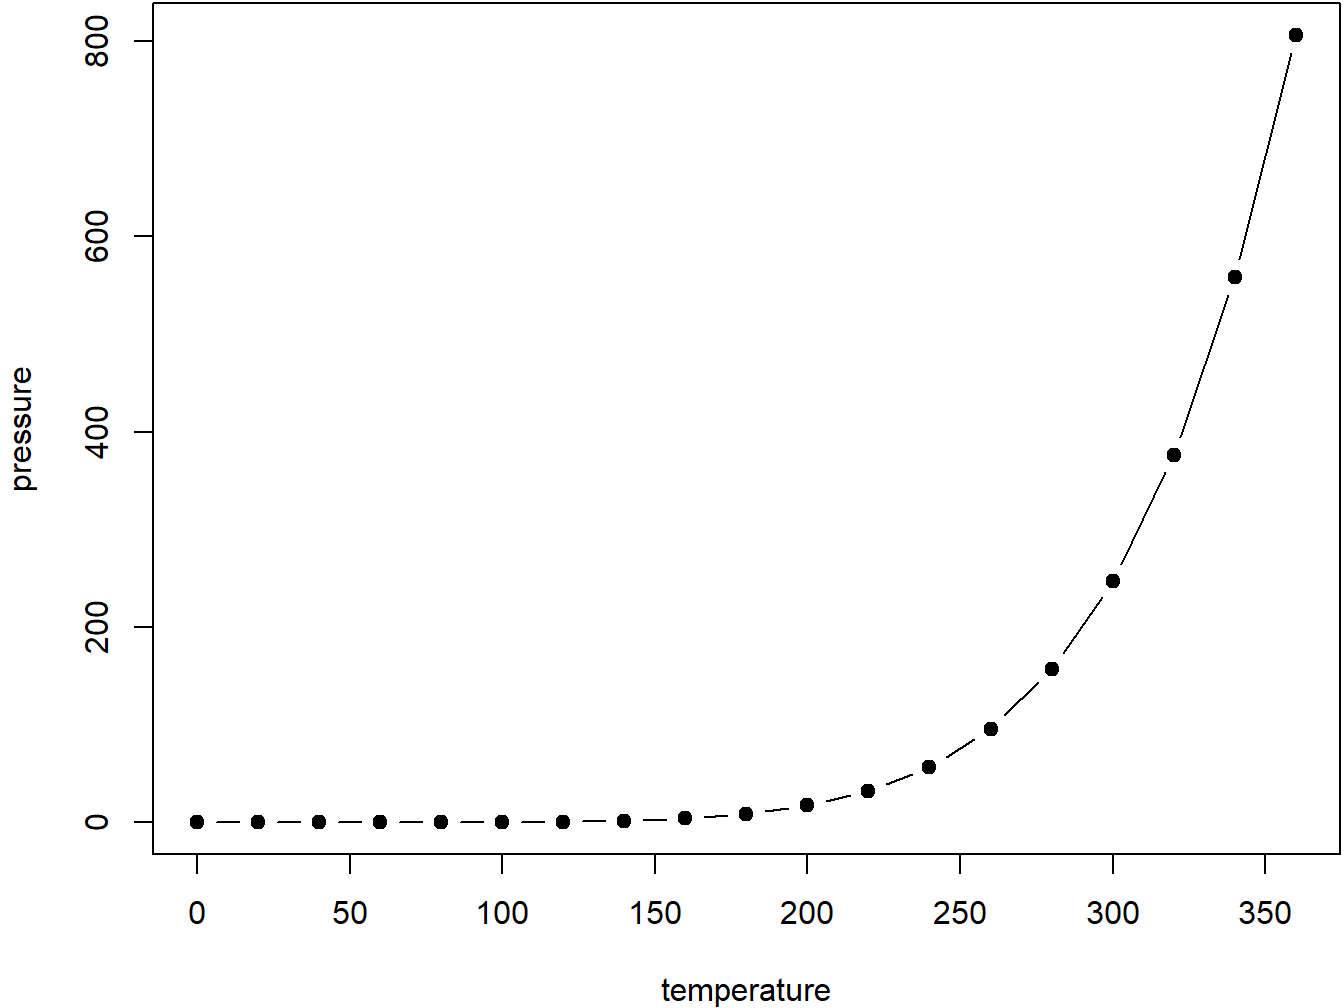
\includegraphics[width=0.8\linewidth]{_main_files/figure-latex/nice-fig-1} 

}

\caption{Here is a nice figure!}\label{fig:nice-fig}
\end{figure}

Don't miss Table \ref{tab:nice-tab}.

\begin{Shaded}
\begin{Highlighting}[]
\NormalTok{knitr}\SpecialCharTok{::}\FunctionTok{kable}\NormalTok{(}
  \FunctionTok{head}\NormalTok{(pressure, }\DecValTok{10}\NormalTok{), }\AttributeTok{caption =} \StringTok{\textquotesingle{}Here is a nice table!\textquotesingle{}}\NormalTok{,}
  \AttributeTok{booktabs =} \ConstantTok{TRUE}
\NormalTok{)}
\end{Highlighting}
\end{Shaded}

\begin{table}

\caption{\label{tab:nice-tab}Here is a nice table!}
\centering
\begin{tabular}[t]{rr}
\toprule
temperature & pressure\\
\midrule
0 & 0.0002\\
20 & 0.0012\\
40 & 0.0060\\
60 & 0.0300\\
80 & 0.0900\\
\addlinespace
100 & 0.2700\\
120 & 0.7500\\
140 & 1.8500\\
160 & 4.2000\\
180 & 8.8000\\
\bottomrule
\end{tabular}
\end{table}

\hypertarget{importance}{%
\chapter{Importance of uncertainty}\label{importance}}

You can add parts to organize one or more book chapters together. Parts can be inserted at the top of an .Rmd file, before the first-level chapter heading in that same file.

Add a numbered part: \texttt{\#\ (PART)\ Act\ one\ \{-\}} (followed by \texttt{\#\ A\ chapter})

Add an unnumbered part: \texttt{\#\ (PART\textbackslash{}*)\ Act\ one\ \{-\}} (followed by \texttt{\#\ A\ chapter})

Add an appendix as a special kind of un-numbered part: \texttt{\#\ (APPENDIX)\ Other\ stuff\ \{-\}} (followed by \texttt{\#\ A\ chapter}). Chapters in an appendix are prepended with letters instead of numbers.

\hypertarget{embracing}{%
\chapter{Embracing uncertainty: The Bayesian approach}\label{embracing}}

\hypertarget{footnotes}{%
\section{Footnotes}\label{footnotes}}

Footnotes are put inside the square brackets after a caret \texttt{\^{}{[}{]}}. Like this one \footnote{This is a footnote.}.

\hypertarget{citations}{%
\section{Citations}\label{citations}}

Reference items in your bibliography file(s) using \texttt{@key}.

For example, we are using the \textbf{bookdown} package \citep{R-bookdown} (check out the last code chunk in index.Rmd to see how this citation key was added) in this sample book, which was built on top of R Markdown and \textbf{knitr} \citep{xie2015} (this citation was added manually in an external file book.bib).
Note that the \texttt{.bib} files need to be listed in the index.Rmd with the YAML \texttt{bibliography} key.

The RStudio Visual Markdown Editor can also make it easier to insert citations: \url{https://rstudio.github.io/visual-markdown-editing/\#/citations}

\hypertarget{Bayesian}{%
\chapter{The Bayesian approach in practice}\label{Bayesian}}

\hypertarget{example-5.2-chronic-obstructive-pulmonary-disease-copd-in-england}{%
\section{Example 5.2: Chronic obstructive pulmonary disease (COPD) in England}\label{example-5.2-chronic-obstructive-pulmonary-disease-copd-in-england}}

We now look at example into the hospital admission rates for chronic obstructive pulmonary disease (COPD) in England between 2001--2010.

In England, there are 324 local authority administrative areas each with an observed and expected number of cases. The expected numbers were calculated using indirect standardisation by applying the age--sex specific rates for the whole of England to the age--sex population profile of each of
the areas.

\hypertarget{reading-in-data-and-shapefiles}{%
\subsection{Reading in data and shapefiles}\label{reading-in-data-and-shapefiles}}

To create SMR maps, we need to read in the relevant shapefiles. The files
\texttt{englandlocalauthority.shp} and \texttt{englandlocalauthority.dbf} contain the location, shape, and attributes of English local authorities. The functions \texttt{read.shp} and \texttt{read.dbf()} will read these shapefiles into \texttt{R}

\begin{Shaded}
\begin{Highlighting}[]
\CommentTok{\# Reading in borders}
\CommentTok{\# copd\_shp \textless{}{-} read.shp(shp.name= "englandlocalauthority.shp")}
\CommentTok{\# copd\_dbf \textless{}{-} read.dbf(dbf.name= "englandlocalauthority.dbf")}
\end{Highlighting}
\end{Shaded}

\hypertarget{example-5.3-fitting-a-poisson-regression-model-in-nimble}{%
\section{Example 5.3: Fitting a Poisson regression model in Nimble}\label{example-5.3-fitting-a-poisson-regression-model-in-nimble}}

\begin{verbatim}
## nimble version 0.12.2 is loaded.
## For more information on NIMBLE and a User Manual,
## please visit https://R-nimble.org.
\end{verbatim}

\begin{verbatim}
## 
## Attaching package: 'nimble'
\end{verbatim}

\begin{verbatim}
## The following object is masked from 'package:stats':
## 
##     simulate
\end{verbatim}

The following code is used to fit the Poisson log-linear model seen in Chapter 2 Section \ldots{} using \texttt{Nimble}

First, define the model in Nimble.

\begin{Shaded}
\begin{Highlighting}[]
\NormalTok{Example5}\FloatTok{.3}\NormalTok{Code }\OtherTok{\textless{}{-}} \FunctionTok{nimbleCode}\NormalTok{(\{}
  \ControlFlowTok{for}\NormalTok{ (i }\ControlFlowTok{in} \DecValTok{1}\SpecialCharTok{:}\NormalTok{N) \{}
\NormalTok{    Y[i] }\SpecialCharTok{\textasciitilde{}} \FunctionTok{dpois}\NormalTok{(mu[i])}
    \FunctionTok{log}\NormalTok{(mu[i]) }\OtherTok{\textless{}{-}} \FunctionTok{log}\NormalTok{(E[i]) }\SpecialCharTok{+}\NormalTok{ beta0 }\SpecialCharTok{+}\NormalTok{ beta1 }\SpecialCharTok{*}\NormalTok{ X1[i] }\SpecialCharTok{+}\NormalTok{ betad }\SpecialCharTok{*}\NormalTok{ X2[i]}
\NormalTok{  \}}
  
  \CommentTok{\# Priors}
\NormalTok{  beta0 }\SpecialCharTok{\textasciitilde{}} \FunctionTok{dnorm}\NormalTok{ (}\DecValTok{0}\NormalTok{ , }\AttributeTok{sd =} \DecValTok{100}\NormalTok{)}
\NormalTok{  beta1 }\SpecialCharTok{\textasciitilde{}} \FunctionTok{dnorm}\NormalTok{ (}\DecValTok{0}\NormalTok{ , }\AttributeTok{sd =} \DecValTok{100}\NormalTok{)}
\NormalTok{  betad }\SpecialCharTok{\textasciitilde{}} \FunctionTok{dnorm}\NormalTok{ (}\DecValTok{0}\NormalTok{ , }\AttributeTok{sd =} \DecValTok{100}\NormalTok{)}
  
  \CommentTok{\# Functions of interest:}
\NormalTok{  base }\OtherTok{\textless{}{-}} \FunctionTok{exp}\NormalTok{(beta0)}
\NormalTok{  RR }\OtherTok{\textless{}{-}} \FunctionTok{exp}\NormalTok{(beta1)}
\NormalTok{\})}
\end{Highlighting}
\end{Shaded}

Read the data and define the constants, data and initials lists for the \texttt{Nimble} model.

\begin{Shaded}
\begin{Highlighting}[]
\NormalTok{data }\OtherTok{\textless{}{-}} \FunctionTok{read.csv}\NormalTok{(}\StringTok{"data/DataExample53.csv"}\NormalTok{, }\AttributeTok{sep =} \StringTok{","}\NormalTok{)}

\NormalTok{ex.const }\OtherTok{\textless{}{-}} \FunctionTok{list}\NormalTok{(}
  \AttributeTok{N =} \DecValTok{393}\NormalTok{,}
  \AttributeTok{E =}\NormalTok{ data}\SpecialCharTok{$}\NormalTok{exp\_lungc65pls,}
  \AttributeTok{X1 =} \FunctionTok{as.vector}\NormalTok{(}\FunctionTok{scale}\NormalTok{(data}\SpecialCharTok{$}\NormalTok{k3)),}
  \AttributeTok{X2 =} \FunctionTok{as.vector}\NormalTok{(}\FunctionTok{scale}\NormalTok{(data}\SpecialCharTok{$}\NormalTok{k2))}
\NormalTok{)}

\NormalTok{ex.data }\OtherTok{\textless{}{-}} \FunctionTok{list}\NormalTok{(}\AttributeTok{Y =}\NormalTok{ data}\SpecialCharTok{$}\NormalTok{lungc65pls)}

\NormalTok{inits }\OtherTok{\textless{}{-}} \ControlFlowTok{function}\NormalTok{()}
  \FunctionTok{list}\NormalTok{(}\AttributeTok{beta0 =} \FunctionTok{rnorm}\NormalTok{(}\DecValTok{1}\NormalTok{),}
       \AttributeTok{beta1 =} \FunctionTok{rnorm}\NormalTok{(}\DecValTok{1}\NormalTok{),}
       \AttributeTok{betad =} \FunctionTok{rnorm}\NormalTok{(}\DecValTok{1}\NormalTok{))}
\end{Highlighting}
\end{Shaded}

Define the parameters' monitors and run the model.

\begin{Shaded}
\begin{Highlighting}[]
\CommentTok{\#parameters to monitor}
\NormalTok{params}\OtherTok{\textless{}{-}}\FunctionTok{c}\NormalTok{(}\StringTok{"beta0"}\NormalTok{,}\StringTok{"beta1"}\NormalTok{,}\StringTok{"betad"}\NormalTok{,}\StringTok{"base"}\NormalTok{,}\StringTok{"RR"}\NormalTok{)}

\NormalTok{samples }\OtherTok{\textless{}{-}} \FunctionTok{nimbleMCMC}\NormalTok{(}
  \AttributeTok{code =}\NormalTok{ Example5}\FloatTok{.3}\NormalTok{Code,}
  \AttributeTok{data =}\NormalTok{ ex.data,}
  \AttributeTok{constants =}\NormalTok{ ex.const,}
  \AttributeTok{inits =}\NormalTok{ inits,}
  \AttributeTok{monitors =}\NormalTok{ params,}
  \AttributeTok{niter =} \DecValTok{22000}\NormalTok{,}
  \AttributeTok{nburnin =} \DecValTok{2000}\NormalTok{,}
  \AttributeTok{thin =} \DecValTok{10}\NormalTok{,}
  \AttributeTok{WAIC =} \ConstantTok{TRUE}\NormalTok{,}
  \AttributeTok{nchains =} \DecValTok{2}\NormalTok{,}
  \AttributeTok{samplesAsCodaMCMC =} \ConstantTok{TRUE}
\NormalTok{)}
\end{Highlighting}
\end{Shaded}

\begin{verbatim}
## Defining model
\end{verbatim}

\begin{verbatim}
## Building model
\end{verbatim}

\begin{verbatim}
## Setting data and initial values
\end{verbatim}

\begin{verbatim}
## Running calculate on model
##   [Note] Any error reports that follow may simply reflect missing values in model variables.
\end{verbatim}

\begin{verbatim}
## Checking model sizes and dimensions
\end{verbatim}

\begin{verbatim}
## Checking model calculations
\end{verbatim}

\begin{verbatim}
## Compiling
##   [Note] This may take a minute.
##   [Note] Use 'showCompilerOutput = TRUE' to see C++ compilation details.
\end{verbatim}

\begin{verbatim}
## Running chain 1 ...
\end{verbatim}

\begin{verbatim}
## |-------------|-------------|-------------|-------------|
## |-------------------------------------------------------|
\end{verbatim}

\begin{verbatim}
## Running chain 2 ...
\end{verbatim}

\begin{verbatim}
## |-------------|-------------|-------------|-------------|
## |-------------------------------------------------------|
##   [Warning] There are individual pWAIC values that are greater than 0.4. This may indicate that the WAIC estimate is unstable (Vehtari et al., 2017), at least in cases without grouping of data nodes or multivariate data nodes.
\end{verbatim}

Check the WAIC.

\begin{Shaded}
\begin{Highlighting}[]
\FunctionTok{str}\NormalTok{(samples)}
\end{Highlighting}
\end{Shaded}

\begin{verbatim}
## List of 2
##  $ samples:List of 2
##   ..$ chain1: 'mcmc' num [1:2000, 1:5] 1.01 1.02 1.01 1.01 1 ...
##   .. ..- attr(*, "dimnames")=List of 2
##   .. .. ..$ : NULL
##   .. .. ..$ : chr [1:5] "RR" "base" "beta0" "beta1" ...
##   .. ..- attr(*, "mcpar")= num [1:3] 1 2000 1
##   ..$ chain2: 'mcmc' num [1:2000, 1:5] 1.002 1.022 1.036 1.031 0.994 ...
##   .. ..- attr(*, "dimnames")=List of 2
##   .. .. ..$ : NULL
##   .. .. ..$ : chr [1:5] "RR" "base" "beta0" "beta1" ...
##   .. ..- attr(*, "mcpar")= num [1:3] 1 2000 1
##   ..- attr(*, "class")= chr "mcmc.list"
##  $ WAIC   :Reference class 'waicList' [package "nimble"] with 7 fields
##   ..$ .CobjectInterface :Formal class 'uninitializedField' [package "methods"] with 2 slots
##   .. .. ..@ field    : chr ".CobjectInterface"
##   .. .. ..@ className: chr "ANY"
##   ..$ .generatorFunction:function (...)  
##   ..$ nimbleListDef     :Reference class 'nimbleListDefClass' [package "nimble"] with 3 fields
##   .. ..$ types     :List of 3
##   .. .. ..$ vars : chr [1:3] "WAIC" "lppd" "pWAIC"
##   .. .. ..$ types: chr [1:3] "double" "double" "double"
##   .. .. ..$ dims : num [1:3] 0 0 0
##   .. ..$ className : chr "waicList"
##   .. ..$ predefined: logi TRUE
##   .. ..and 14 methods.
##   ..$ nestedListGenList : list()
##   ..$ WAIC              : num 3049
##   ..$ lppd              : num -1514
##   ..$ pWAIC             : num 10.2
##   ..and 17 methods, of which 3 are  possibly relevant:
##   ..  initialize, initialize#nimbleListBase, show#envRefClass
\end{verbatim}

\begin{Shaded}
\begin{Highlighting}[]
\NormalTok{samples}\SpecialCharTok{$}\NormalTok{WAIC}
\end{Highlighting}
\end{Shaded}

\begin{verbatim}
## nimbleList object of type waicList
## Field "WAIC":
## [1] 3049.375
## Field "lppd":
## [1] -1514.449
## Field "pWAIC":
## [1] 10.23901
\end{verbatim}

Show the traceplots and posterior summaries for each of the parameters.

\begin{Shaded}
\begin{Highlighting}[]
\NormalTok{mvSamples }\OtherTok{\textless{}{-}}\NormalTok{ samples}\SpecialCharTok{$}\NormalTok{samples}

\CommentTok{\#trace plots of beta1}
\FunctionTok{plot}\NormalTok{(mvSamples[, }\FunctionTok{c}\NormalTok{(}\StringTok{"beta1"}\NormalTok{)])}
\end{Highlighting}
\end{Shaded}

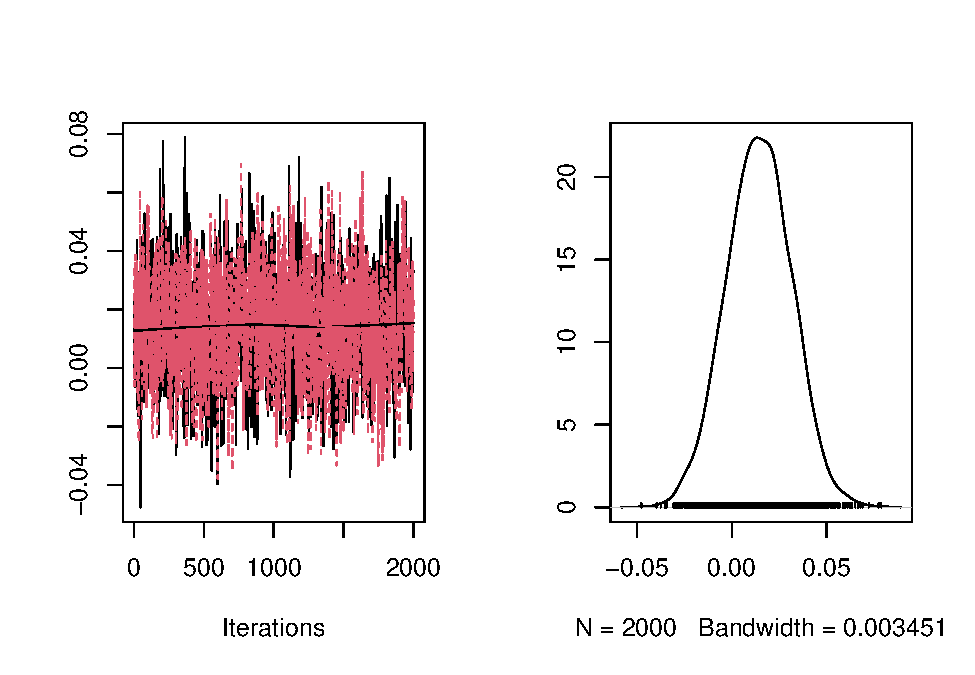
\includegraphics{_main_files/figure-latex/Ex 5.3 traceplots-1.pdf}

\begin{Shaded}
\begin{Highlighting}[]
\CommentTok{\#trace plots of base}
\FunctionTok{plot}\NormalTok{(mvSamples[, }\FunctionTok{c}\NormalTok{(}\StringTok{"base"}\NormalTok{)])}
\end{Highlighting}
\end{Shaded}

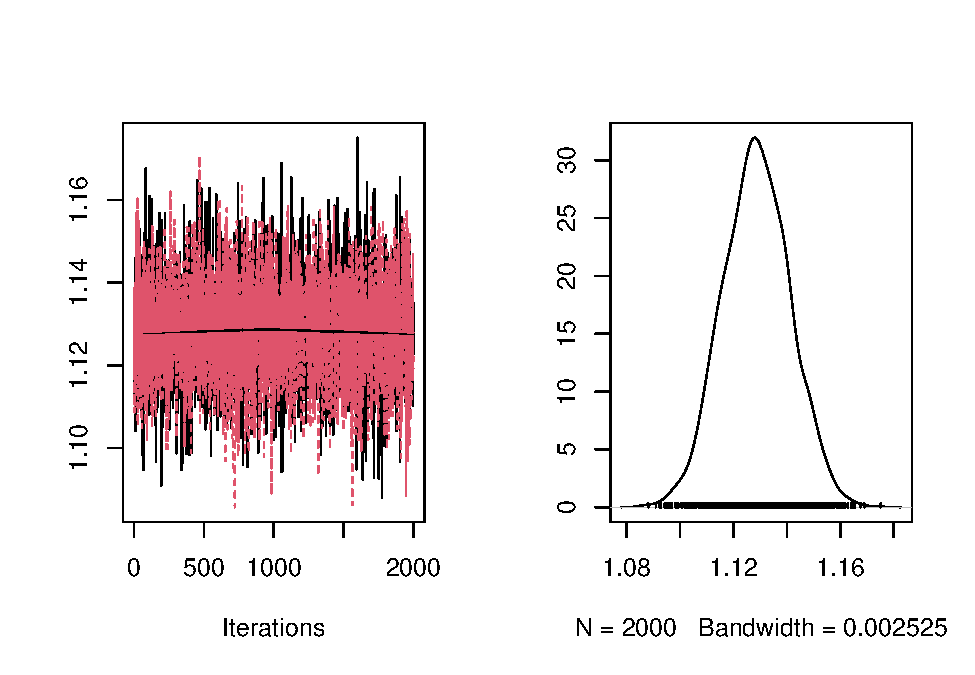
\includegraphics{_main_files/figure-latex/Ex 5.3 traceplots-2.pdf}

\begin{Shaded}
\begin{Highlighting}[]
\CommentTok{\#trace plots of RR}
\FunctionTok{plot}\NormalTok{(mvSamples[, }\FunctionTok{c}\NormalTok{(}\StringTok{"RR"}\NormalTok{)])}
\end{Highlighting}
\end{Shaded}

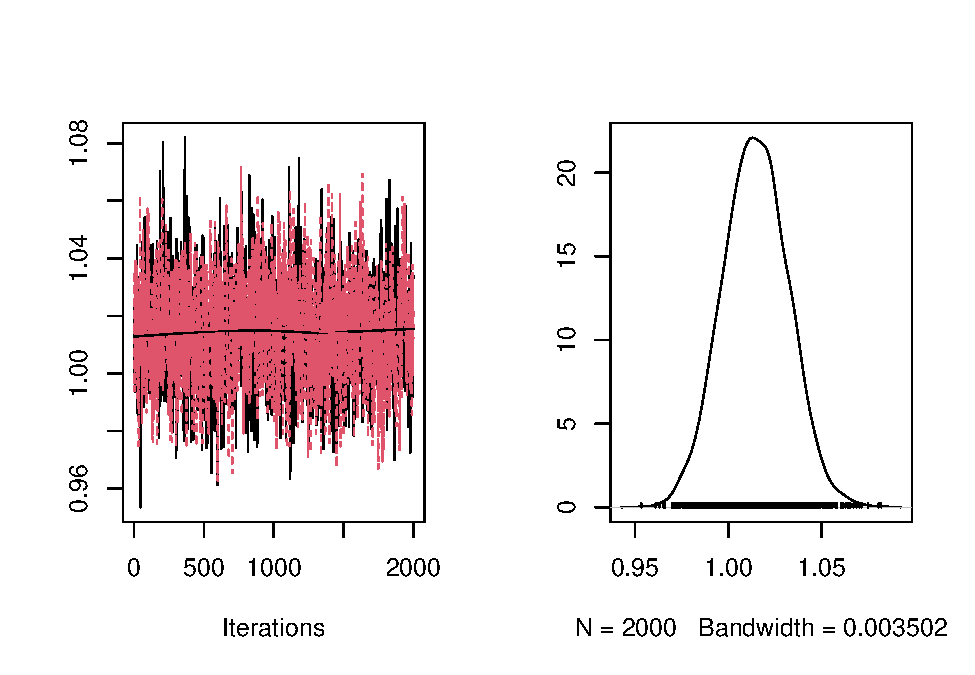
\includegraphics{_main_files/figure-latex/Ex 5.3 traceplots-3.pdf}

\begin{Shaded}
\begin{Highlighting}[]
\CommentTok{\#posterior summary of base}
\FunctionTok{summary}\NormalTok{(mvSamples[, }\FunctionTok{c}\NormalTok{(}\StringTok{"base"}\NormalTok{)])}
\end{Highlighting}
\end{Shaded}

\begin{verbatim}
## 
## Iterations = 1:2000
## Thinning interval = 1 
## Number of chains = 2 
## Sample size per chain = 2000 
## 
## 1. Empirical mean and standard deviation for each variable,
##    plus standard error of the mean:
## 
##           Mean             SD       Naive SE Time-series SE 
##      1.1285928      0.0125133      0.0001979      0.0001979 
## 
## 2. Quantiles for each variable:
## 
##  2.5%   25%   50%   75% 97.5% 
## 1.105 1.120 1.129 1.137 1.153
\end{verbatim}

\begin{Shaded}
\begin{Highlighting}[]
\CommentTok{\#posterior summary of RR}
\FunctionTok{summary}\NormalTok{(mvSamples[, }\FunctionTok{c}\NormalTok{(}\StringTok{"RR"}\NormalTok{)])}
\end{Highlighting}
\end{Shaded}

\begin{verbatim}
## 
## Iterations = 1:2000
## Thinning interval = 1 
## Number of chains = 2 
## Sample size per chain = 2000 
## 
## 1. Empirical mean and standard deviation for each variable,
##    plus standard error of the mean:
## 
##           Mean             SD       Naive SE Time-series SE 
##      1.0146846      0.0173715      0.0002747      0.0004316 
## 
## 2. Quantiles for each variable:
## 
##   2.5%    25%    50%    75%  97.5% 
## 0.9812 1.0030 1.0146 1.0262 1.0485
\end{verbatim}

\hypertarget{sharing-your-book}{%
\chapter{Sharing your book}\label{sharing-your-book}}

\hypertarget{publishing}{%
\section{Publishing}\label{publishing}}

HTML books can be published online, see: \url{https://bookdown.org/yihui/bookdown/publishing.html}

\hypertarget{pages}{%
\section{404 pages}\label{pages}}

By default, users will be directed to a 404 page if they try to access a webpage that cannot be found. If you'd like to customize your 404 page instead of using the default, you may add either a \texttt{\_404.Rmd} or \texttt{\_404.md} file to your project root and use code and/or Markdown syntax.

\hypertarget{metadata-for-sharing}{%
\section{Metadata for sharing}\label{metadata-for-sharing}}

Bookdown HTML books will provide HTML metadata for social sharing on platforms like Twitter, Facebook, and LinkedIn, using information you provide in the \texttt{index.Rmd} YAML. To setup, set the \texttt{url} for your book and the path to your \texttt{cover-image} file. Your book's \texttt{title} and \texttt{description} are also used.

This \texttt{gitbook} uses the same social sharing data across all chapters in your book- all links shared will look the same.

Specify your book's source repository on GitHub using the \texttt{edit} key under the configuration options in the \texttt{\_output.yml} file, which allows users to suggest an edit by linking to a chapter's source file.

Read more about the features of this output format here:

\url{https://pkgs.rstudio.com/bookdown/reference/gitbook.html}

Or use:

\begin{Shaded}
\begin{Highlighting}[]
\NormalTok{?bookdown}\SpecialCharTok{::}\NormalTok{gitbook}
\end{Highlighting}
\end{Shaded}


  \bibliography{book.bib}

\end{document}
